\chapter{Task-Based, Parallel and Distributed Kirchhoff Seismic Pre-Stack Depth Migration Application \label{chap:exp_km}}
\graphicspath{{chapters/exp_kirchhoff/}}


In this chapter the Kirchhoff seismic pre-stack depth migration is implemented with several task based programming models.
The definition of the tasks is also introduced in this chapter.
Moreover, we will also perform numerical experiments on supercomputers as well as discuss the results obtained from these experiments.

\section{Algorithms}
In this section, the algorithms for the  Kirchhoff seismic pre-stack depth migration will be introduced.
To begin with, the basic algorithm of the method will be presented.
Then, multi-grid algorithms will be introduced.
Finally, parallelism in the method will be discussed and task based algorithms will be shown.

\subsection{Basic Algorithm}

Algorithm \ref{alg:first_look} is the basic and most simple algorithm of the Kirchhoff seismic pre-stack depth migration.
It is a basis on which the other algorithms are founded.


\begin{algorithm}[h]
	\DontPrintSemicolon
	\SetAlgoVlined
	\caption{Kirchhoff Migration \label{alg:first_look}}
	\ForEach{trace $t_{S,R}$}{
		Read the source S and the receiver R from $t_{S,R}$. \;
		\ForEach{point P(x,y,z) of the image}{
			Compute the travel time $Ts$ between $S$ and $P$ (using Green functions)\;
			Compute the travel time $Tr$ between $P$ and $R$ (using Green functions)\;
			Compute the amplitude $A_{S,R}(x,y,z)$.\;
			$im(x,y,z)=im(x,y,z) + A_{S,R}(x,y,z) \cdot t_{S,R}(Ts + Tr)$
		}
	}
\end{algorithm}

\begin{algorithm}[h]
	\DontPrintSemicolon
	\SetAlgoVlined
	\caption{Kirchhoff Migration with coarse and fine grids\label{alg:kirchhoff_multigrids}}
	\ForEach{trace t}{
		\ForEach{(x, y, z) in the coarse grid CG}{
			r = extractR(t)\;
			s = extractS(t)\;
			CG(x, y, z).TS(s) = computeTravelTimeFromVelocityModel(s, x, y, z)\;
			CG(x, y, z).TR(r) = computeTravelTimeFromVelocityModel(r, x, y, z)\;
			CG(x, y, z).A(s,r) = computeAmplitude(s, r, x, y, z)\;
			\ForEach{(i, j, k) in the fine grid FG}{
				CG(x, y, z).FG(i, j, k).TS(s) = interpolateTime(i, j, k, CG(x, y, z).TS(s), CG(x + 1, y, z).TS(s), CG(x - 1, y, z).TS(s), CG(x, y + 1, z).TS(s), CG(x, y - 1, z).TS(s), CG(x, y, z + 1).TS(s), CG(x, y, z - 1).TS(s))\;
				CG(x, y, z).FG(i, j, k).TR(r) = interpolateTime(i, j, k, CG(x, y, z).TR(r), CG(x + 1, y, z).TR(r), CG(x - 1, y, z).TR(r), CG(x, y + 1, z).TR(r), CG(x, y - 1, z).TR(r), CG(x, y, z + 1).TR(r), CG(x, y, z - 1).TR(r))\;
				CG(x, y, z).FG(i, j, k).A(s,r) = interpolateAmplitude(i, j, k, CG(x, y, z).A(s,r), CG(x + 1, y, z).A(s,r), CG(x - 1, y, z).A(s,r), CG(x, y + 1, z).A(s,r), CG(x, y - 1, z). A(s,r), CG(x, y, z + 1).A(s,r), CG(x, y, z - 1).A(s,r))\;
				CG(x, y, z).FG(i, j, k).v += CG(x, y, z).FG(i, j, k).A(s, r) x ts,r(CG(x, y, z).FG(i, j, k).TS(s) + CG(x, y, z).FG(i, j, k).TR(r))\;
			}
		}
	}
\end{algorithm}

Algorithm \ref{alg:first_look} is computationally bound since the computation of the travel time between $S$ and $R$ through $P$ takes a long time.
Indeed, the travel time is computed by using Green functions which are heavy to compute from the initial velocity model.
In practice two optimisations are used : multi-grids and pre-computation of the Green functions.

Algorithm \ref{alg:kirchhoff_multigrids} illustrates the use of two grids.
In the multi-grids approach, the travel time is computed for the coarse grid then interpolated for the fine grid.
The travel time for each point of the fine grid is interpolated from the travel time computed for the coarse grid.


\begin{algorithm}[h]
	\DontPrintSemicolon
	\SetAlgoVlined
	\caption{Kirchhoff Migration with multi-grids and loading precomputed Green functions \label{alg:kirchhoff_mg+load}}
	\ForEach{trace t}{
		\ForEach{(x, y, z) in the coarse grid CG}{
			r = extractR(t)\;
			s = extractS(t)\;
			Gs = loadPrecomputedGreenFunc(s)\;
			Gr = loadPrecomputedGreenFunc(r)\;
			CG(x, y, z).TS(s) = computeTravelTimeFromGreenFunc(Gs, x, y, z)\;
			CG(x, y, z).TR(r) = computeTravelTimeFromGreenFunc(Gr, x, y, z)\;
			CG(x, y, z).A(s,r) = computeAmplitude(s, r, x, y, z)\;
			\ForEach{(i, j, k) in the fine grid FG}{
				CG(x, y, z).FG(i, j, k).TS(s) = interpolateTime(i, j, k, CG(x, y, z).TS(s), CG(x + 1, y, z).TS(s), CG(x - 1, y, z).TS(s), CG(x, y + 1, z).TS(s), CG(x, y - 1, z).TS(s), CG(x, y, z + 1).TS(s), CG(x, y, z - 1).TS(s))\;
				CG(x, y, z).FG(i, j, k).TR(r) = interpolateTime(i, j, k, CG(x, y, z).TR(r), CG(x + 1, y, z).TR(r), CG(x - 1, y, z).TR(r), CG(x, y + 1, z).TR(r), CG(x, y - 1, z).TR(r), CG(x, y, z + 1).TR(r), CG(x, y, z - 1).TR(r))\;
				CG(x, y, z).FG(i, j, k).A(s,r) = interpolateAmplitude(i, j, k, CG(x, y, z).A(s,r), CG(x + 1, y, z).A(s,r), CG(x - 1, y, z).A(s,r), CG(x, y + 1, z).A(s,r), CG(x, y - 1, z). A(s,r), CG(x, y, z + 1).A(s,r), CG(x, y, z - 1).A(s,r))\;
				CG(x, y, z).FG(i, j, k).v += CG(x, y, z).FG(i, j, k).A(s, r) x ts,r(CG(x, y, z).FG(i, j, k).TS(s) + CG(x, y, z).FG(i, j, k).TR(r))\;
			}
		}
	}
\end{algorithm}

Algorithm \ref{alg:kirchhoff_mg+load} shows the use of the two optimisations.
The two grids are used and the Green functions are loaded from the file system.

\subsection{Parallelism}
In the Kirchhoff Migration, only the output image is modified.
The traces and the Green functions are accessed only for reading.
Therefore, the update of the image by the contribution of a trace conditions the parallelism available.
Moreover, the traces are independent and the update of a point of the image depends only on the contribution of the trace.

It leans that \textbf{all the points can be updated at the same time by a trace}.
It also means that there is concurrency problems if a point is updated by two traces.
Actually, since the update is a sum, it is worth considering to create images for different sets of traces independently then reduce (sum) the different images into a final image.

From a computational point of view, traces can be treated in any order and points can be computed independently.
Several traces can be treated at the same time with reductions on the output images.
So there is a lot of available computational parallelism but there is also data to transfer between compute units and from the file system.
Moreover, creating several images to reduce them later also produces communications to reunite them into one.
In the case where the Green functions are precomputed, loading them into the memory can be an issue.
They take a lot of space on disk so it is expensive to load them several times.

Thus, scheduling those data movements can be a good alternative to find an efficient way to manage the data without having to communicate too much.
In order to better express the dependencies, the method is described as a graph of tasks.

\subsection{Task algorithm}

The algorithms are rewritten to allow the use of tasks.
Basically, functions were created and those functions will be the tasks that will be used.
The task algorithm is the Algorithm \ref{alg:kirchhoff_task} and the function associated can be found in the Algorithm \ref{alg:kirchhoff_task_def}.

\begin{algorithm}[h]
	\DontPrintSemicolon
	\SetAlgoVlined
	\caption{Task Kirchhoff Migration \label{alg:kirchhoff_task}}
	\ForEach{trace t}{
		\ForEach{(x, y, z) in the coarse grid CG}{
			r = extractR(t)\;
			s = extractS(t)\;
			Gs = loadPrecomputedGreenFunc(s)\;
			Gr = loadPrecomputedGreenFunc(r)\;
			CG(x, y, z).TS(s) = computeTravelTimeFromGreenFunc(Gs, x, y, z)\;
			CG(x, y, z).TR(r) = computeTravelTimeFromGreenFunc(Gr, x, y, z)\;
			CG(x, y, z).A(s,r) = computeAmplitude(s, r, x, y, z)\;
			updateFineGrid(CG(x, y, z), CG(x + 1, y, z).TS(s), CG(x - 1, y, z).TS(s), CG(x, y + 1, z).TS(s), CG(x, y - 1, z).TS(s), CG(x, y, z + 1).TS(s), CG(x, y, z - 1).TS(s), CG(x + 1, y, z).TR(r), CG(x - 1, y, z).TR(r), CG(x, y + 1, z).TR(r), CG(x, y - 1, z).TR(r), CG(x, y, z + 1).TR(r), CG(x, y, z - 1).TR(r), CG(x + 1, y, z).A(s,r), CG(x - 1, y, z).A(s,r), CG(x, y + 1, z).A(s,r), CG(x, y - 1, z). A(s,r), CG(x, y, z + 1).A(s,r), CG(x, y, z - 1).A(s,r))\;
		}
	}
\end{algorithm}

In Algorithm \ref{alg:kirchhoff_task}, the tasks on the blocks of the coarse grid for a given trace can be executed in parallel.

\begin{algorithm}[h]
	\DontPrintSemicolon
	\SetAlgoVlined
	\caption{Task definition for Kirchhoff Migration \label{alg:kirchhoff_task_def}}
	\SetKwProg{Fn}{Task}{is}{end}

	\Fn{updateFineGrid(B:current block:inout;\;
	TSu, TSb, TSr, TSl, TSf, TSh:TravelTime;in\;
	TRu, TRb, TRr, TRl, TRf, TRh:TravelTime;in\;
	TSu, TSb, TSr, TSl, TSf, TSh:Amplitude;in)}{
		\ForEach{(i, j, k) in the fine grid FG}{
			B.FG(i, j, k).TS(s) = interpolateTime(i, j, k, B.TS(s), TSu, TSb, TSr, TSl, TSf, TSh)\;
			B.FG(i, j, k).TR(r) = interpolateTime(i, j, k, B.TR(r), TRu, TRb, TRr, TRl, TRf, TRh)\;
			B.FG(i, j, k).A(s,r) = interpolateAmplitude(i, j, k, B.A(s,r), TSu, TSb, TSr, TSl, TSf, TSh)\;
			B.FG(i, j, k).v += B.FG(i, j, k).A(s, r) $\times$ ts,r(B.FG(i, j, k).TS(s) + B.FG(i, j, k).TR(r))\;
		}
	}
\end{algorithm}

In Algorithm \ref{alg:kirchhoff_task_def}, the loop on the elements of the fine grid can also be executed in parallel.
There is at least two level of parallelism.


\subsection{Use of GPUs}
This section aims to add the use of GPUs in the Kirchhoff seismic pre-stack depth migration.
GPUs are slower than CPUs but there a lot more computing unit in GPUs.
They are used to process huge amount of parallel operations and they are very useful to perform simple operations on huge amount of data.
Therefore, most of the operations inside the fine grid can be performed on GPU since the operations are the same on all the data.
Indeed, the operation is a linear combination of several arrays at the same point.

\subsection{Pre-fetching and spreading the data}
Since the main issue is the communications between the storage system where the Green functions are and the computing units inside the super-computer, a solution would be to pre-fetch the data.
The Green functions would be stored in a storage system closer of the computing unit and faster.
It is possible to efficiently predict which Green function will be needed by the program when the source and the receiver of the trace are loaded.

Moreover, two block side by side share the Green functions at their frontier.
That means the same Green functions are loaded several times in a short amount of time from the file system.
The bandwidth between the file system and the computing unit is generally lower than the one between two nodes of the super-computer so use them will be more efficient.
To do so, the pre-fetcher will be modified to become aware of the tasks that uses the Green functions.
Then, if the Green function a task may want is still loaded in another task, the task using the Green function will send it to the task that also need it.
It will reduce the communications to the file system containing the Green functions and so, make the whole process faster.

To go further, a computing node of the super-computer may be able to store some of the Green functions even if it does not use them in order to provide them to the other nodes as long as possible.

\section{2D Implementation}

For this implementation, we simplified the Kirchhoff seismic pre-stack depth migration by considering the absorption to be equal to 1 and by only studying the 2D case.
This application is available at \url{https://github.com/jgurhem/KirchhoffMigration}.

\subsection{C Kernel Description}
The kernel performing the main operations for this method is implemented in C and provide functions to manage traces, Green functions and images.
There is three kind of functions implemented in this kernel.
The first type is IOs to read and write traces, images and Green functions from files.
The second type of function is used to associate propagation time precomputed with Green functions to the trace that will be used to create the image.
Then, the last type is the actual migration.

The migration function expect a fine grain image to update and a trace with the propagation times to make the round trip from the source of the trace to the receiver passing by every point of the large grain image.
It performs an interpolation to compute the propagation time needed to travel from the source to the receiver for each point of the fine grain image by using the propagation times shipped with the trace.
So, with the knowledge of the time it would take to make the round trip to the considered image point, we scale it to the trace time scale in order to retrieve the amplitude of the sound wave at this time in the trace.
Then, the amplitude is added to the value at the corresponding point in the fine grain image.
This amplitude could be scaled with the absorption at this point but we set the absorption to 1 for this implementation so this is not necessary here.
The migration function has OpenMP directives to parallelize the work on the image.
They can be activated by compiling the library with OpenMP.

For our experiments, we use a use constant velocity model to generate the initial propagation times.
Therefore, we implemented a function to interpolate propagation times on a large grain grid from the constant velocity model.
A function to generate simple traces has also been implemented to use in our experiments.

\begin{figure}[h]
	\centering
	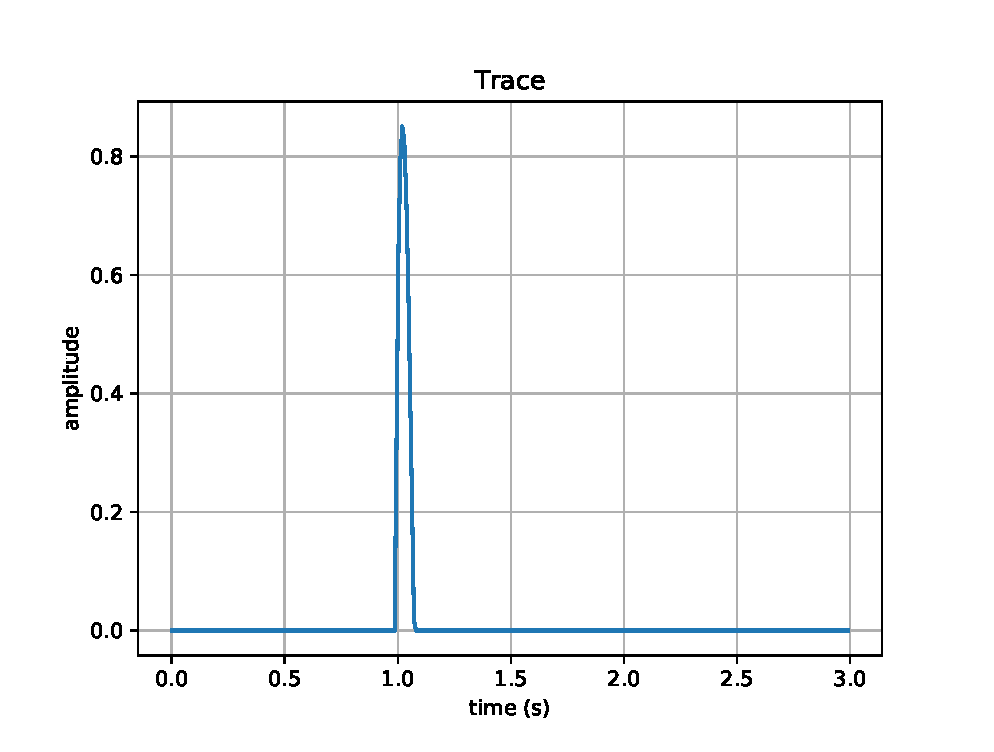
\includegraphics[width=.7\textwidth]{trace}
	\caption{Trace example\label{fig:kirchhoff_trace}}
\end{figure}

Figure \ref{fig:kirchhoff_trace} gives an example of a generated trace used to test the 2D application with these simplifications.
This trace used as test and is not used in our experiments.

\begin{figure}[H]
	\centering
	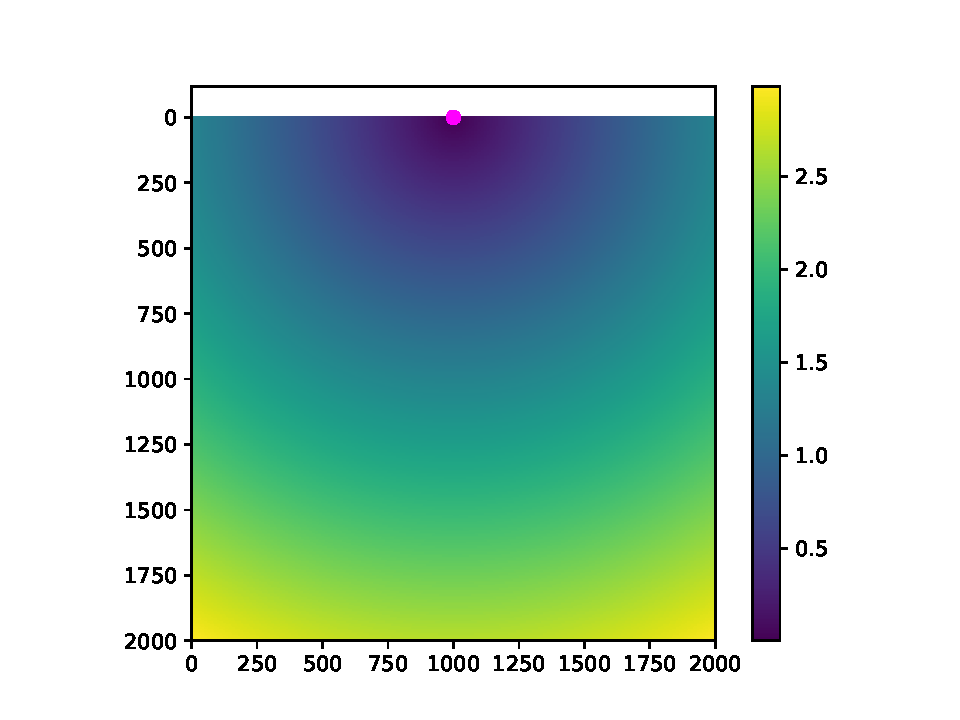
\includegraphics[width=.7\textwidth]{trace1000ppt.pdf}
	\caption{Propagation times for a source and receiver at the same place\label{fig:kirchhoff_pt}}
\end{figure}

Figure \ref{fig:kirchhoff_pt} is a plot of the propagation times to make the round trip from the source point located at (1000,0), each point of the figure and the receiver located at (1000, 0) in a uniform middle.

\begin{figure}[H]
	\centering
	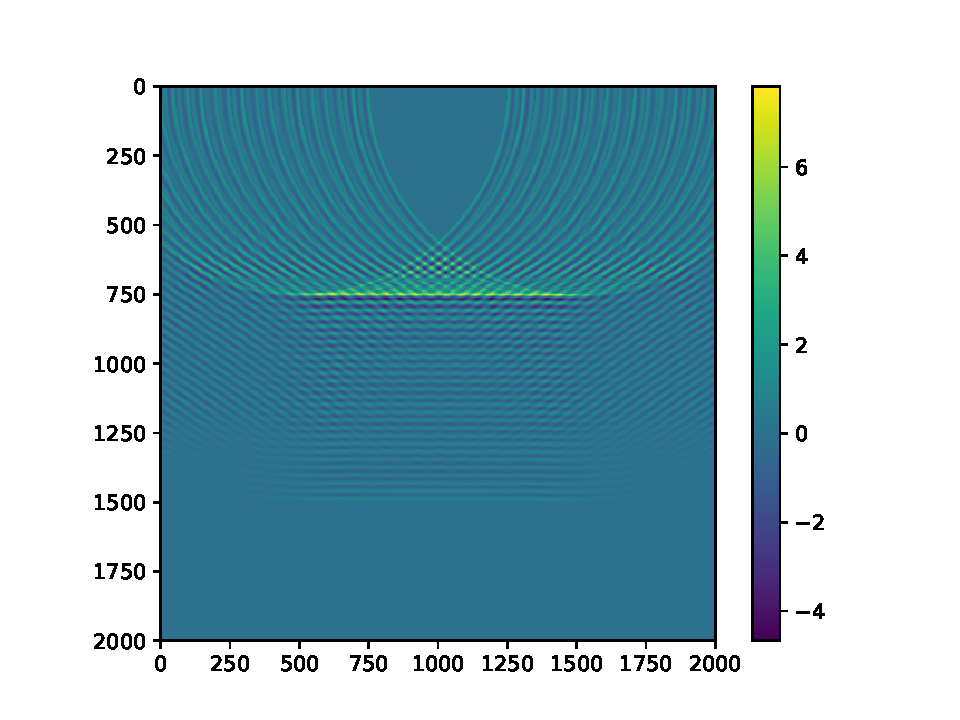
\includegraphics[width=.7\textwidth]{img.pdf}
	\caption{Image obtained from a migrated trace\label{fig:kirchhoff_image}}
\end{figure}
Figure \ref{fig:kirchhoff_image} is the migrated image produced by the Kirchhoff migration with the trace of Figure \ref{fig:kirchhoff_trace} taken at several different source locations (the source and the receiver are located at the same place).

\subsection{Distributed and Parallel Applications}
Distributed and parallel applications were implemented on top of the C kernel in MPI and HPX.

The MPI application uses the C functions to generate the traces and propagation time associated on the distributed processes.
The image is distributed across the processes allocated to the application.
The traces are duplicated on each process since they will be accessed depending on the travel time extracted from the propagation time shipped with the trace.
The propagation times are generated with the trace and only the part that will be used in the migration is selected.
Then, the migration can be executed on the local image with the local trace and propagation times.

The HPX application is based on same principles.
The image is split and managed by tasks.
A task calling the migration available in the kernel has been implemented as well as tasks to generate the traces and the propagation times.
There is also tasks to associate the trace with the appropriate propagation times.

These applications support the generation and processing of several traces.
They were designed to perform scaling experiments on the migration with a distributed image.

\section{2D Numerical Experiments}
In this section, we perform numerical experiments on the Kirchhoff seismic pre-stack depth migration implemented in MPI, MPI+OpenMP and HPX on Pangea II.
We perform strong scaling and weak scaling experiments as well as we study the influence of the number of OpenMP threads on our kernel.

\subsection{Strong Scaling}
Strong scaling experiments were performed on a 15000 $\times$ 15000 points image.
We executed our Kirchhoff seismic pre-stack depth migration MPI, MPI+OpenMP and HPX applications on 10 generated traces with propagation times.
We study the performances improvement of the migration while the number of nodes (cores) increases and the size of the image is kept constant.

\begin{figure}[H]
        \centering
        \includegraphics[width=.45\textwidth]{{{fig_pangea2_ss_nx15000_ny15000}}}
        \includegraphics[width=.45\textwidth]{{{fig_pangea2_ss2_nx15000_ny15000}}}

        \caption{Strong scaling considering HPX, MPI and MPI+OpenMP for a 15000 $\times$ 15000 points image on Pangea II. Legend is (model). \label{fig:km:pangea2_ss}}
\end{figure}

Figure \ref{fig:km:pangea2_ss} shows the results of our strong scaling experiments on the Kirchhoff seismic pre-stack depth migration for a image of size of 15000 $\times$ 15000 and 10 traces.
HPX execution times are increasing with the increase of computing resources which should not be the case.
This may be due to the internal management of the memory in HPX as we have to convert the C data structures in C++ data structures that HPX can work with since the applications use the same kernel to perform the computations but the performances are different than MPI's.
Moreover, HPX may induce image migration between nodes that are not necessary.
MPI+OpenMP has issues when scaling from 2 to 4 nodes but scales well from 4 to 8.
It has performances close to MPI, especially for 8 nodes.
MPI has the best performances and also scales well.
The applications use the same kernel but the management of the memory is up to the programming model used to implement the application.
This explain the difference of performances between MPI and HPX.
As for the differences between MPI and MPI+OpenMP, the OpenMP directives introduced in the kernel does not seem to take advantage of the cores available on the nodes since we use 4 processes per nodes and 6 OpenMP threads per process.

\subsection{Weak Scaling}
Weak scaling experiments were performed on a image which number of points increases with the number of nodes used.
The base image size is 15000 $\times$ 15000 and the first dimension is multiplied by the number of nodes.
For instance, the image used for 4 nodes is 60000 $\times$ 15000.
We executed our Kirchhoff seismic pre-stack depth migration MPI, MPI+OpenMP and HPX applications on 10 generated traces with propagation times.
We study the performances improvement of the migration while the number of nodes (cores) and the size of the image increases.

\begin{figure}[H]
        \centering
        \includegraphics[width=.45\textwidth]{{{fig_pangea2_ws_nx15000_ny15000}}}
        \includegraphics[width=.45\textwidth]{{{fig_pangea2_ws2_nx15000_ny15000}}}

        \caption{Weak scaling considering HPX, MPI and MPI+OpenMP for a 15000 $\times$ 15000 points image on Pangea II. Legend is (model). \label{fig:km:pangea2_ws}}
\end{figure}

Figure \ref{fig:km:pangea2_ws} shows the results of our weak scaling experiments on the Kirchhoff seismic pre-stack depth migration for a image of base size of 15000 $\times$ 15000 which grows with the number of nodes (cores) and 10 traces.
The ideal weak scaling is a constant execution time when the computing resources allocated to the application are increasing in the same proportions as the data.
This is not the case for HPX.
This may be due to HPX memory management and unexpected image and trace migrations between nodes which we are not able to control.
MPI+OpenMP weak scaling the almost perfect until 8 nodes where there is a issue and the execution time is abnormally high.
The MPI application has a weak scaling almost perfect.

\subsection{Variation of the Number of OpenMP Threads}
Experimentations on the MPI+OpenMP Kirchhoff seismic pre-stack depth migration application with different number of OpenMP threads allocated to the application have been performed for an image of 15000 $\times$ 15000 points.
On one hand, we used only one process and changed the number of OpenMP threads allocated to the application until all the cores of the node are used.
On the other hand, we used all the cores of the node but we changed the number of processes allocated to the MPI+OpenMP as well as the number of OpenMP threads allocated per process in order to keep one thread per core.

\begin{table}[H]
	\centering
	\begin{tabular}{ccc}
\hline
Threads& Cores& Median\\
\hline
2& 24& 63.383\\
4& 24& 65.3781\\
6& 24& 71.5322\\
12& 24& 76.7288\\
24& 24& 254.1039\\
\hline
\end{tabular}

	\caption{Execution time for a pure OpenMP application while increasing the number of OpenMP threads allocated to the application for a 15000 $\times$ 15000 point image on Pangea II. \label{tab:km:omp_testp1}}
\end{table}

Table \ref{tab:km:omp_testp1} shows the execution times depending on the number of threads allocated to the pure OpenMP application on one node of Pangea II.
We can see that the execution time does not change while increasing the number of threads except for 24 threads where it is very high.
This shows that the OpenMP directives introduced in the kernel does not produce multi-threaded code that takes advantage of the available cores.

\begin{table}[H]
	\centering
	\begin{tabular}{cccc}
\hline
Processes& Cores& Median& Threads\\
\hline
2& 24& 46.7809& 12\\
4& 24& 6.3982& 6\\
6& 24& 4.3045& 4\\
12& 24& 8.7822& 2\\
24& 24& 2.0901& 1\\
\hline
\end{tabular}

	\caption{Execution time for a hybrid MPI+OpenMP application while increasing the number of MPI process while keeping 24 OpenMP threads allocated to the application for a 15000 $\times$ 15000 point image. \label{tab:km:omp_testpm}}
\end{table}

Table \ref{tab:km:omp_testpm} shows the execution times for the MPI+OpenMP executed on one node of Pangea II where all the cores run an OpenMP thread and the number of MPI processes changes.
The number of thread allocated for each MPI process is the number of cores (24) divided by the number of MPI processes allocated to the application.
We can clearly see that the pure MPI application (24 processes and 1 thread per process) is the fastest case.
There is also two unexpected values ; for 4 processes with 6 threads per process and for 12 processes with 2 threads per process.
These values does not line up with the rest.
Especially the value for 12 processes with 2 threads per process that should reasonably be between the value for 6 and 24 processes.

In conclusion of our scaling experiments on the implementations of the Kirchhoff seismic pre-stack depth migration, our HPX application does not scale very well both in term of weak and strong scaling compared to our MPI application.
In the MPI application, the location of each piece of data can be exactly controlled and there are no communications during the migration.
On the contrary, the data migrations in our HPX application are up to the runtime of the programming model.
Therefore, there may be migration of the images and the traces across the nodes which reduce the performances.
Moreover, there is a conversion between the C data structures used in the C kernel and the C++ data structure used in HPX that may also decrease the performances of the application since the data are not converted in the C based MPI application.
Finally, the introduction of OpenMP directives in the kernel is not successful since the performances are not improved with an hybrid MPI+OpenMP implementation compared to a pure MPI implementation.

% chapter transition
\paragraph{}
In this chapter, we introduced the experiments we made with the parallel and distributed sparse matrix vector product we implemented using the selected task based programming models.
We also discussed the numerical experiments we performed and the results we obtained.
The experiments and the studies made with the tasks based programming models allowed the selection of key features for the task based programming models.
We will resume these key features and how they are expressed in the task based programming models in the following chapter.